\documentclass[12pt]{article}
\usepackage[letterpaper]{geometry}
\usepackage{amsmath, amsthm, amssymb, amsfonts}
\usepackage{graphicx}
\usepackage{titling}
\usepackage{hyperref}
\newcommand{\subtitle}[1]{%
  \posttitle{%
    \par\end{center}
    \begin{center}\large#1\end{center}
    \vskip0.5em}%
}
\hypersetup{
    colorlinks=true,
    linkcolor=blue,
    filecolor=magenta,      
    urlcolor=blue,
} 
\urlstyle{same}
\title{CSE 180 - Robotics \\ Final Project}
\subtitle{Team Alpha}
\author{Christine Breckenridge, Aleksandr Brodskiy, Carlos Martinez}
\begin{document}
\maketitle
{\setlength{\parindent}{0cm}
\textbf{Outline}
\begin{enumerate}  
\item Documentation
\item Design Decisions
\item Team Member Work-Log
    \item Conclusion\\\\\\\\\\\\\\\\\\\\\\\\\\\\\\\\\\
\end{enumerate} 
}
{\setlength{\parindent}{0cm}
\textbf{Documentation} \\
\paragraph{} In order to develop a complete and efficient solution of detecting treasures within an arbitrary map of consistent dimensions, an approach was devised such that the computations performed by the various, specialized algorithms would be distributed.
  In this manner, the implementation of this approach involved the creation of three nodes, \textbf{\textit{nav.cpp}}, \textbf{\textit{planner.cpp}}, and \textbf{\textit{treasures.cpp}}.
  \begin{center} \textit{see the} \textbf{Design Decisions} \textit{section for further detail regarding optimizations}. \end{center}
  \paragraph{} The primary data structures utilized in the formulization of this distributed approach were a one dimensional array as well as a map with a \textbf{\textit{string}} type as the key and a \textbf{\textit{pose}} object as the value.
  The simplification of storing a \textbf{\textit{pose}} object within the map was predominantly related to its dependance on the ROS structs \textit{\textbf{point}} and \textit{\textbf{quaternion}} for the computing of the translation and rotation of the husky robot, respectively.
  The instantiation of the map constructor is demonstrated below with the \textbf{\textit{treasures}} label:
  \begin{center} \textsc{std\textbf{::}map< char[], Pose > \textbf{\textit{treasures}}} \end{center}  
  \paragraph{} Furthermore, by subscribing to the \textit{map} topic it became possible to retrieve data embedded in the ROS message:
  \begin{center} \textsc{nav\_msgs/OccupancyGrid} \end{center}
  \paragraph{} This message contains the \textsc{Header header}, \textsc{MapMetaData info} , and \textsc{int}8\_\textsc{t}[] \textsc{data} fields. The \textsc{MapMetaData info} field provides information regarding the height, width, and resolution of the environment map.
  The height, width, and resolution are defined as follows:
  \begin{center} \textsc{unsigned int} \textsc{height} \\ \textsc{unsigned int} \textsc{width} \\ \textsc{float} \textsc{resolution} \end{center}
  \paragraph{}With these objects and data structures, the launch file created for the execution of the three nodes provided the husky robot with the ability to concurrently plan a path while scanning for treasures and traversing the environment. The latter two operations in tandem are the most computationally intensive programs of this endeavor. 
  \\\\
}
{\setlength{\parindent}{0cm}
\textbf{Design Decisions} 
\\\\ \textit{the following screenshot exemplifies the husky robot's inability to plan a navigable path when there is considerable error in the localization.} 
\begin{center} 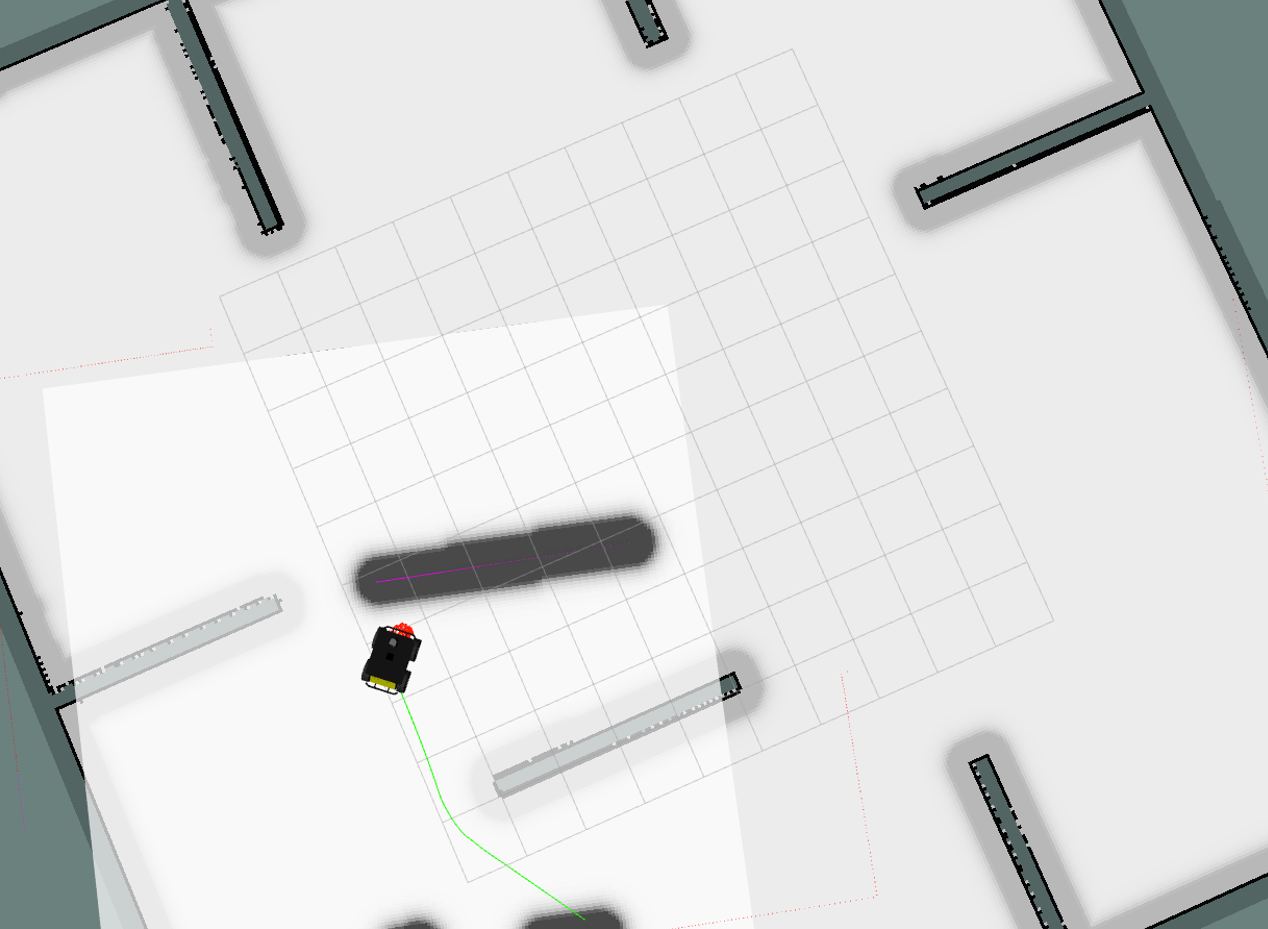
\includegraphics[width=120mm]{RViz1.png} \end{center}
\textit{as is observable from the screenshot, the husky robot is unable to differentiate between its estimated position and that of the physical barrier. This causes rotational discrepancies which lead to collisions with the environment.}
\paragraph{} In order to ameliorate the inconsistent accuracy of the husky robot's localization estimations, the inflation radius was increased. 
  The utilization of inflation radius within the cost map enabled the avoidance of collisions with the environment . Essentially, this was the most prominent design decision as it was carefully speculated to prevent the husky robot from, as previously stated, colliding with obstacles present within the environment.   
\\\\\\\\\\  
}
{\setlength{\parindent}{0cm}
\textbf{Testing/QA}\\
\begin{center}\underline{Treasures}\end{center}
\paragraph{}Global coordinates of the treasures dispersed about the map were computed with a transformation by utilizing the \textbf{\textit{tf}}2 transform listener. By looking up the transformation between the \textbf{\textit{map}} and the \textsc{logical\_camera\_link} frame the global coordinates of the treasure were calculated. 
  The aforementioned \textsc{map} data structure was updated with each newly, non$-$redundant, found treasure. The returned pose was compared to the predefined pose to ensure validity of the computed data. As such, the mathematical integrity of the solutions implemented in \textbf{\textit{treasures.cpp}} were verified and consequently published to the respective listeners. 
\begin{center}\underline{Navigation}\end{center}
\paragraph{}During the process of developing an efficient \textit{\textbf{nav.cpp}}, a timeout waiting period of 15 and 45 seconds was introduced in order to delay the sending of the next goal point to the husky robot. This was done in order to prevent the husky robot from prematurely traversing the map before arriving at the corner$-$most location of the map.
  In this manner the quality control aspect of this node was primarily ensured with a trial$-$and$-$error method of arriving at a reasonable timeout waiting period. Therefore the husky robot is able to begin traversing the environment from the corner$-$most location of the map.  
\begin{center}\underline{Planner}\end{center}
\paragraph{}The \textbf{\textit{x\_dist}}, \textbf{\textit{y\_dist}}, and \textbf{\textit{obstacle\_dist}} variables were utilized to demarcate distances along the x-axis and y-axis between points, respectively, as well as the minimum distance from obstacles. In testing, the values of these parameters were refined in order to obtain the desired behavior. The goal was to have the husky robot traverse the entire map to find the treasures without getting too close to obstacles so as to avoid  collisions.
\\\\ 
}
{\setlength{\parindent}{0cm}
\textbf{Conclusion}
\paragraph{}Upon completing the endeavor of traversing a treasure$-$\textit{filled} map, a direct solution was implemented with respect to the planning, navigation, and treasure detection of the husky robot. Along with this, an indirect solution was implemented to mitigate the inaccuracy of the \textsc{AMCL} algorithm. 
\end{document} 


